% 2015 LHCb leptonic tau decay
LHCb has published two measurements of \RDst/; one measurement from 2015 where
the $\tau$ is reconstructed leptonically in the \TauLepMode/ decay mode, and
another from 2018 where the $\tau$ is reconstructed in the \TauHadMode/ decay.

The 2015 result constituted the first \RDst/ measurement in the very challenging
environment of a hadron collider.
This analysis is heavily inspired by the previous $B$ factory measurements, with
a few key differences:

\begin{itemize}
    \item The $B \bar{B}$ rest frame is unknown.
    \item Larger backgrounds, especially a significant contribution due to the
        following decay mode: $B \rightarrow \Dst/ H_c X$, where $H_c$ is any
        charm meson, and $X$ is any hadronic particle.
        These decay modes have similar $m^2_{miss}$ and $E^{*}_l$ distributions
        very similar to the signal.
    \item A particular decay mode of the $B$ and \Dst/ are chosen so that all
        visible final state particles are charged due to the fact that the
        neutral particle resolution is not very good.
\end{itemize}

Without the $B \bar{B}$ rest frame, the tagging algorithms used in the $B$
factory measurements cannot be applied.
This problem is solved by the so-called \emph{rest frame approximation}, a
technique developed specifically for this analysis.
This approximation assumes the momentum of the $B$ that is orthogonal to the
beam axis, transverse momentum, is unchanged.
The component of the $B$ momentum parallel to the beam axis, $(p_{B})_z$, is
approximated as
\begin{equation}
    (p_{B})_z = \frac{m_B}{m_{reco}} (p_{reco})_z,
\end{equation}
with $m_B$ being the known $B$ mass, and $reco$ referring to the $\Dst/ \mu^-$
system.
The resulting $m^2_{miss}$ resolution is worse than that of the $B$ factories,
but is sufficient to preserve the discriminating power between the signal and
normalization, as shown in \autoref{fig:babar_lhcb_fit_comparison}.

A multivariate method is employed to determine which tracks are likely to have
originated from the $B_{sig}$ decay.
Events that contain tracks that are not associated with the \Dst/ or the
$\mu^-$ are rejected, reducing the $B \rightarrow \Dst/ H_c X$ and other
backgrounds.
By inverting the isolation selecting criteria, control samples are obtained to
correct for the shape of these background distributions.

An extended, binned, maximum likelihood method is used in the fit, with three
dimensional templates in the $m^2_{miss}$, $E^*_\mu$, and $q^2$ variables
describing the contributions from signal, normalization, and background events.
\autoref{fig:babar_lhcb_fit_comparison} (g, h, i) show the fit results.
We see that this LHCb result has a lower signal-to-background ratio, but
significantly higher number of signal events.

\begin{figure}[ht]
    \centering
    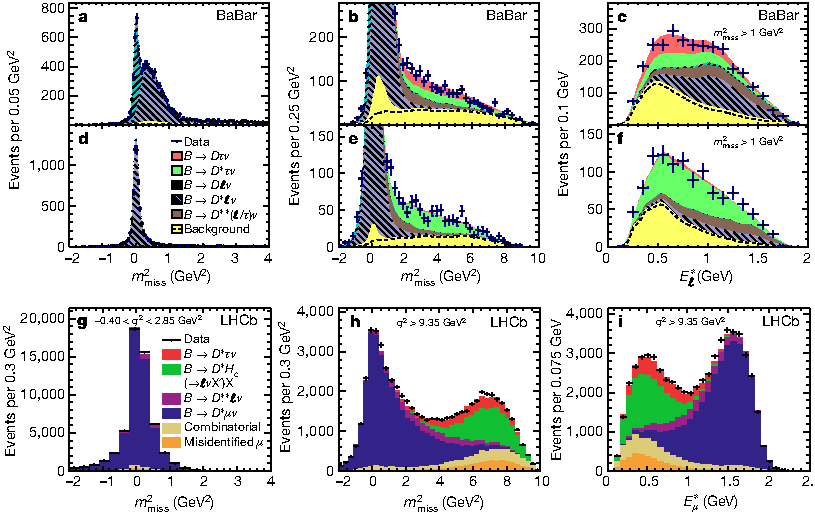
\includegraphics[width=0.85\textwidth]{figs/babar_lhcb_fit_comparison.pdf}
    \caption{
        Comparison between fitted data between 2013 \BaBar/ and 2015
        LHCb result \cite{Ciezarek:2017yzh}.
    }
    \label{fig:babar_lhcb_fit_comparison}
\end{figure}

% 2018 LHCb hadronic tau decay: tau -> pi pi pi
The 2018 LHCb \RDst/ measurement pioneered the usage of \TauHadMode/ decay modes
in \BDstMode{\tau}.

Since the $\tau$ lepton is reconstructed with the hadronic modes, the final
state particles of signal events are different from those of normalization
events.
Instead, to cancel experimental systematic uncertainties, this analysis employs
the $B \rightarrow \Dst/ 3\pi$ as the normalization, which has the same final
state particles as that of the signal.
This analysis measures the ratio, defined as $\mathcal{K}(\Dst/))$
\begin{equation}
    \mathcal{K}(D^{*-}) \equiv \frac{
        \mathcal{B}(\BDstMode{\tau})
    }{
        \mathcal{B}(B \rightarrow \Dst/ 3 \pi)
    },
\end{equation}
which can be converted back to \RDst/ with the appropriate branching fractions.

This analysis took a different approach to separate signal from normalization
events:
With the decay mode \TauHadMode/,
the $\tau$ decay vertex can be reconstructed from the intersection of the three
charged pion tracks.
Due to the non-zero lifetime of the $\tau$, its decay vertex is separated from
the $B$ meson decay vertex.
In contrast, the three pions from the $B \rightarrow \Dst/ \pi \pi \pi X$
normalization (prompt) mode come directly from the $B$ decay vertex.
By requiring a clear separation between the two vertices, the normalization mode
can be effectively separated from signal events, as \autoref{fig:lhcb_3pi_topo}
shows.
The main background is composed of $B \rightarrow \Dst/ D X$ double-charm events,
which is suppressed by a specifically-designed multivariate method.

\begin{figure}[ht]
    \centering
    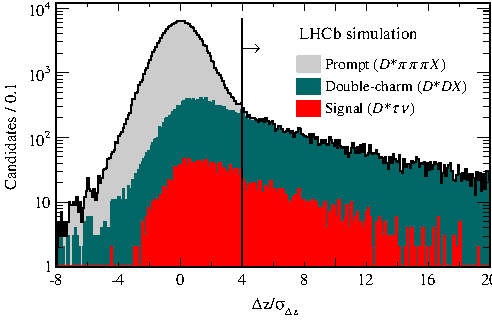
\includegraphics[width=0.65\textwidth]{figs/lhcb_3pi_topo.pdf}
    \caption{
        Separations between the $B$ decay vertex and a secondary vertex,
        possibly $\tau$ decay vertex, in the signal, the normalization, and the
        background decay mode, indicating different topologies between these
        modes \cite{Aaij:2017deq}.
    }
    \label{fig:lhcb_3pi_topo}
\end{figure}

This measurement, which uses the hadronic $\tau$ decays, results in a
significantly reduced statistical uncertainty compared to the 2015 LHCb result.
However the total uncertainty is dominated by systematic effects.
